\documentclass[../../main.tex]{subfiles}
\begin{document}

\begin{flushright}
\footnotesize\textit{【自動文字起こし・要確認】}
\end{flushright}

{\bf [解1]}
対称性から，$A(1,0)$，$B(\cos\alpha,\sin\alpha)$，$C(\cos\beta,\sin\beta)$（$0<\alpha\le\pi$，$\alpha<\beta<2\pi$）としてよい．
\begin{align}
|AB|^2&=(\cos\alpha-1)^2+\sin^2\alpha=2(1-\cos\alpha)=4\sin^2\dfrac{\alpha}{2}\\
|BC|^2&=(\cos\beta-\cos\alpha)^2+(\sin\beta-\sin\alpha)^2=2\{1-(\cos\alpha\cos\beta+\sin\alpha\sin\beta)\}=2(1-\cos(\beta-\alpha))\\
|CA|^2&=2(1-\cos\beta)=4\sin^2\dfrac{\beta}{2}
\end{align}
である．$P=|AB|^2+|BC|^2+|CA|^2$とおく．

\paragraph{(1)}
\begin{align}
P>8&\iff\cos\alpha+\cos\beta+\cos(\beta-\alpha)<-1\\
&\iff2\cos\dfrac{\alpha}{2}\cos\left(\beta-\dfrac{\alpha}{2}\right)<-2\cos^2\dfrac{\alpha}{2}\quad\cdots①
\end{align}
である．$\alpha=\pi$の時①は$0<0$となって不適だから，$0<\alpha<\pi$である．この時$\cos\dfrac{\alpha}{2}>0$だから，
\begin{align}
①&\iff\cos\left(\beta-\dfrac{\alpha}{2}\right)<\cos\left(\pi-\dfrac{\alpha}{2}\right)\\
&\iff\left(\pi-\dfrac{\alpha}{2}\right)+2n\pi<\beta-\dfrac{\alpha}{2}<\left(\pi+\dfrac{\alpha}{2}\right)+2n\pi\quad(n\in\mathbb Z)\\
&\iff\pi+2n\pi<\beta<(\pi+\alpha)+2n\pi
\end{align}

$0<\beta<2\pi$から，$n=0$で
\begin{align}
①\iff\pi<\beta<\pi+\alpha\iff\triangle ABC\text{は鋭角三角形}
\end{align}

よって，示された．

\begin{figure}[htb]
\centering
\begin{tikzpicture}[scale=1.8, >=stealth]
  \coordinate (O) at (0,0);
  \draw (O) circle (1);
  \coordinate (A) at (1,0);
  \coordinate (B) at (137:1);
  \coordinate (C) at (280:1);
  \draw (A) -- (B) -- (C) -- (A);
  \draw[gray, dashed] (O) -- (A);
  \draw[gray, dashed] (O) -- (B);
  \fill (O) circle (0.4pt) node[below left] {\scriptsize $O$};
  \fill (A) circle (0.5pt) node[right] {$A$};
  \fill (B) circle (0.5pt) node[above left] {$B$};
  \fill (C) circle (0.5pt) node[below] {$C$};
  \draw pic["\scriptsize $\alpha$", draw, angle radius=8mm] {angle=A--O--B};
\end{tikzpicture}
\caption{単位円に内接する$\triangle ABC$}
\end{figure}

\paragraph{(2)}
\begin{align}
P\le9\iff-\dfrac{3}{2}\le\cos\alpha+\cos\beta+\cos(\beta-\alpha)\quad\cdots②
\end{align}
である．この右辺を$f(\beta)$とおく．$t=\cos\dfrac{\alpha}{2}$とすると，$0<t<1$で，
\begin{align}
f(\beta)=2t\cos\left(\beta-\dfrac{\alpha}{2}\right)+2t^2-1\quad\cdots③
\end{align}
であり，これは$\cos(\beta-\alpha/2)$の単調増加関数で，$\beta=\pi+\dfrac{\alpha}{2}$（$\alpha<\beta<2\pi$を満たす）で最小値
\begin{align}
f(\beta)=2t^2-2t-1
\end{align}
をとる．次に$t$で平方完成して
\begin{align}
f(\beta)=2\left(t-\dfrac{1}{2}\right)^2-\dfrac{3}{2}
\end{align}
だから②は示された．等号成立は$t=\dfrac{1}{2}$かつ$\beta=\pi+\dfrac{\alpha}{2}$の時で，$0<\alpha<\pi$だから$\alpha=\dfrac{2}{3}\pi$，$\beta=\dfrac{4}{3}\pi$

つまり$\triangle ABC$は正三角形である．

\bigskip
\noindent{\bf [解2]}
右のおりがく．$\triangle ABC$の外接円の半径は$1$だから，正弦定理から，
\begin{align}
|AB|=2\sin C,\quad|BC|=2\sin A,\quad|CA|=2\sin B
\end{align}
たから$P=4(\sin^2A+\sin^2B+\sin^2C)$である．

\begin{figure}[htb]
\centering
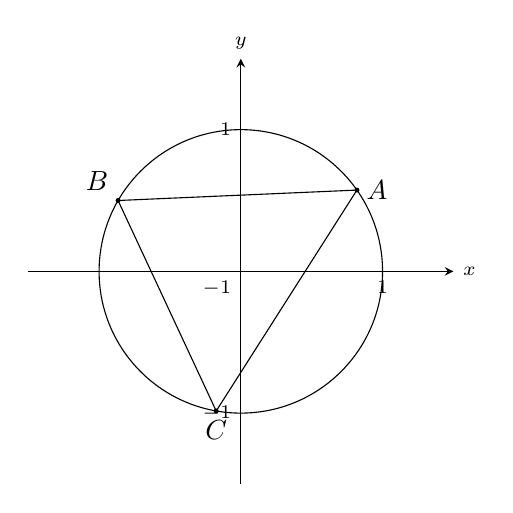
\begin{tikzpicture}[scale=1.8, >=stealth]
  \draw[->] (-1.5,0) -- (1.5,0) node[right] {\scriptsize $x$};
  \draw[->] (0,-1.5) -- (0,1.5) node[above] {\scriptsize $y$};
  \draw (0,0) circle (1);
  \coordinate (A) at (35:1);
  \coordinate (B) at (150:1);
  \coordinate (C) at (260:1);
  \draw (A) -- (B) -- (C) -- (A);
  \fill (A) circle (0.5pt) node[right] {$A$};
  \fill (B) circle (0.5pt) node[above left] {$B$};
  \fill (C) circle (0.5pt) node[below] {$C$};
  \node[below left] {\scriptsize $-1$};
  \node[below] at (1,0) {\scriptsize $1$};
  \node[left] at (0,1) {\scriptsize $1$};
  \node[left] at (0,-1) {\scriptsize $-1$};
\end{tikzpicture}
\caption{正弦定理による別解}
\end{figure}

\paragraph{(1)}
\begin{align}
\dfrac{1}{2}P&=\sin^2A+\sin^2B+\sin^2(\pi-A-B)\\
&=\dfrac{1-\cos2A}{2}+\dfrac{1-\cos2B}{2}+\dfrac{1-\cos2(A+B)}{2}
\end{align}
\begin{align}
\dfrac{1}{2}P&=3-\{\cos2A+\cos2B+\cos2(A+B)\}\\
&=3-\{2\cos(A+B)\cos(A-B)+2\cos^2(A+B)-1\}\\
&=4-2\cos(A+B)\{\cos(A-B)+\cos(A+B)\}\\
&=4-4\cos(A+B)\cos A\cos B
\end{align}

だから，
\begin{align}
P>8\iff\cos(A+B)\cos A\cos B<0\iff\cos A\cos B\cos C>0
\end{align}
（$\because\cos(A+B)=\cos(\pi-C)=-\cos C$）である．$\cos A,\cos B,\cos C$のうち2つが負であるとすると，例えば$B,C$が鈍角となって$B+C>\pi$となり，$0<A$，$A+B+C=\pi$に反するので，$\cos A,\cos B,\cos C>0$となり$\triangle ABC$は鋭角三角形．

\paragraph{(2)}
\begin{align}
\dfrac{1}{2}P&=3-\{\cos2A+\cos2B+\cos2C\}\\
&=3-\{2t^2-1+2\cos(A+B)\cos(A-B)\}\quad(t=\cos C)\\
&=4-\{2t^2-2\cos(A-B)\cdot t\}\quad(\because A+B+C=\pi\text{より}\cos(A+B)=-t)\\
&=4+\dfrac{1}{2}\cos^2(A-B)-2\left\{t-\dfrac{1}{2}\cos(A-B)\right\}^2
\end{align}

だから，
\begin{align}
P=8+\cos^2(A-B)-4\left\{t-\dfrac{1}{2}\cos(A-B)\right\}^2\le9
\end{align}

等号成立は$\cos(A-B)=\pm1$かつ$t=\dfrac{1}{2}\cos(A-B)$の時で，$-\pi<A-B<\pi$だから
\begin{align}
\cos(A-B)=1,\quad t=\dfrac{1}{2}\quad\therefore\ A=B=C=\dfrac{\pi}{3}
\end{align}

\newpage

\end{document}
